\documentclass[a4paper, 12pt]{article}
    \usepackage[portuges]{babel}
    \usepackage[utf8]{inputenc}
    \usepackage{amsmath}
    \usepackage{indentfirst}
    \usepackage{graphicx}
    \usepackage{placeins}
    \usepackage{multicol,lipsum}
    \usepackage{indentfirst}
    \setlength{\parindent}{0.6cm}
    \newcommand\tab[1][0.6cm]{\hspace*{#1}}
        
        
    \begin{document}
    \sloppy
    \begin{titlepage}
      \begin{center}
          \Huge{Universidade Federal de Pernambuco}\\
          \large{Deep Logic Networks: Inserting and Extracting
    Knowledge From Deep Belief Networks}\\ 
          \vspace{15pt}
          \vspace{95pt}
          \textbf{\LARGE{Relatório}}\\
          \vspace{3,5cm}
      \end{center}
    
      \begin{flushleft}
          \begin{tabbing}
                      José Nilton\\
                      Italo Paulino\\
                      Mateus Gonçalves\\ 
                      Wallace Soares\\
          \end{tabbing}
      \end{flushleft}
      \vspace{1cm}
    
      \begin{center}
          \vspace{\fill}
          Junho - 2018\\
      \end{center}
    \end{titlepage}
    \newpage
    \tableofcontents
    \thispagestyle{empty}
    \newpage
    \pagenumbering{arabic}
    \section{Introdução}
    O uso de redes \textit{deep} para resolução de problemas complexos envolvendo \textit{Big Data} vem sendo cada vez mais comum nas ultimas décadas. Entretanto compreender o treinamento deste tipo de rede não é trivial. Áreas como a \textit{neural-symbolic computing} estudam em como o conhecimento pode ser inserido e extraido de redes neurais \textit{deep} \cite{Tran}, \cite{garbook}, \cite{garConf}. Através da inserção de conhecimento Tran e Garcez \cite{Tran} mostraram que é possível economizar tempo de processamento pois tal inserção já será uma alternativa a fase de pré-treinamento.
    Já a extração de conhecimento é importante por duas razões: compreensão e re-inserção de conhecimento. Compreender como cada unidade da rede esta se especializando em cada \textit{feature} do padrão de entrada. Re-inserção pois uma vez em que sabemos como cada unidade se especializou em cada \textit{feature} podemos modificar o conhecimento da rede para melhor seu treinamento.
    
    Tran e Garcez\cite{Tran} propõem no artigo em análise um método de inserção e extração de conhecimento em \textit{Deep Belief Networks} - DBNs. DBNs são definidas como n-Restricted Boltzman Machines - RBMs empilhadas de forma que a camada de escondida de uma RBM seja a camada visivel da próxima como mostra a figura abaixo. Exploramos os conceitos de RBMs e DBNs nas seções 1.1 e 1.2, respectivamente.
    
    \begin{figure}[h]
     \centering
     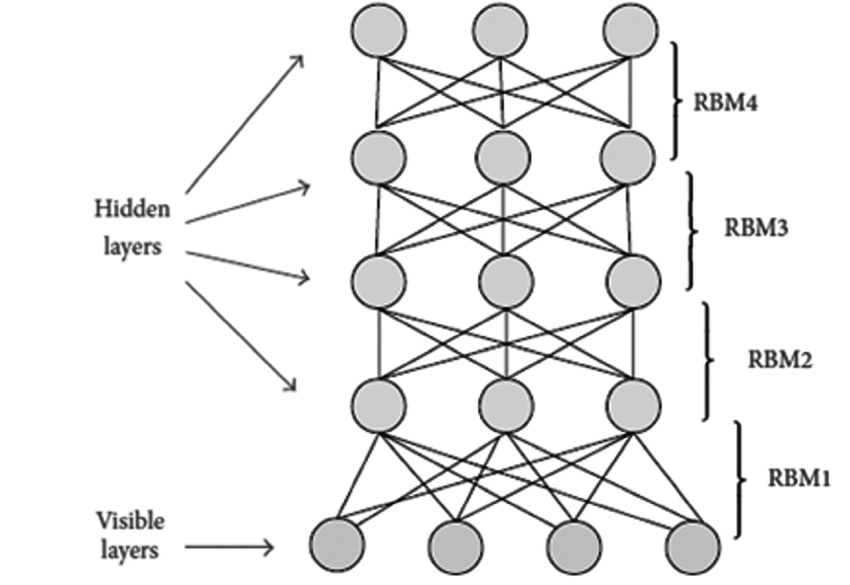
\includegraphics[scale=0.3]{Graphical-Representation-of-a-Deep-Belief-Network.png}
     \caption{Representação gráfica de \textit{Deep Belief Networks}.\cite{imagem1}}
    \end{figure}
    
    \subsection{Restricted Boltzman Machines}
    RBMs constituem-se por neurônios que formam grafos bidirecionais que ligam a camada visivel à camada escondida. O objetivo desta rede é aproximar ao máximo o resultado da camada escondida com o que esta sendo apresentado na entrada. Lidar com este tipo de treinamento que gera uma probabilidade do padrão de saida ser igual ao padrão de entrada se faz necessário pois a maioria dos dados existentes não estão categorizados. Entretando, RBMs podem ser utilizadas tanto para aprendizado supervisionado ou não-supervisionado. Como definido por \cite{overviewRBM}, RBMs são modelos baseados em energia, isto é para cada estado que a RBM possuir, uma energia será associada e assim um probalidade da rede estar representando o padrão de entrada.
    \subsection{Deep Beliefs Networks}
    DBNs são essencialmente várias RBMs empilhadas onde, como dito na introdução, a camada escondida de uma RBM será a camada visível da próxima, e assim sucessivamente.
    
    \subsection{Regras de Confidência}
    
    \section{Motivação}
    \section{Implementação}
    \section{Modulos}
    \section{Metodologia de comparação dos resultados}
    \section{Conclusão}
    \bibliographystyle{ieeetr}
    \bibliography{sample}
    \end{document}
        
        
        
        
        
        
        
    No newline at end of file
    
    